\documentclass[1p]{elsarticle_modified}
%\bibliographystyle{elsarticle-num}

%\usepackage[colorlinks]{hyperref}
%\usepackage{abbrmath_seonhwa} %\Abb, \Ascr, \Acal ,\Abf, \Afrak
\usepackage{amsfonts}
\usepackage{amssymb}
\usepackage{amsmath}
\usepackage{amsthm}
\usepackage{scalefnt}
\usepackage{amsbsy}
\usepackage{kotex}
\usepackage{caption}
\usepackage{subfig}
\usepackage{color}
\usepackage{graphicx}
\usepackage{xcolor} %% white, black, red, green, blue, cyan, magenta, yellow
\usepackage{float}
\usepackage{setspace}
\usepackage{hyperref}

\usepackage{tikz}
\usetikzlibrary{arrows}

\usepackage{multirow}
\usepackage{array} % fixed length table
\usepackage{hhline}

%%%%%%%%%%%%%%%%%%%%%
\makeatletter
\renewcommand*\env@matrix[1][\arraystretch]{%
	\edef\arraystretch{#1}%
	\hskip -\arraycolsep
	\let\@ifnextchar\new@ifnextchar
	\array{*\c@MaxMatrixCols c}}
\makeatother %https://tex.stackexchange.com/questions/14071/how-can-i-increase-the-line-spacing-in-a-matrix
%%%%%%%%%%%%%%%

\usepackage[normalem]{ulem}

\newcommand{\msout}[1]{\ifmmode\text{\sout{\ensuremath{#1}}}\else\sout{#1}\fi}
%SOURCE: \msout is \stkout macro in https://tex.stackexchange.com/questions/20609/strikeout-in-math-mode

\newcommand{\cancel}[1]{
	\ifmmode
	{\color{red}\msout{#1}}
	\else
	{\color{red}\sout{#1}}
	\fi
}

\newcommand{\add}[1]{
	{\color{blue}\uwave{#1}}
}

\newcommand{\replace}[2]{
	\ifmmode
	{\color{red}\msout{#1}}{\color{blue}\uwave{#2}}
	\else
	{\color{red}\sout{#1}}{\color{blue}\uwave{#2}}
	\fi
}

\newcommand{\Sol}{\mathcal{S}} %segment
\newcommand{\D}{D} %diagram
\newcommand{\A}{\mathcal{A}} %arc


%%%%%%%%%%%%%%%%%%%%%%%%%%%%%5 test

\def\sl{\operatorname{\textup{SL}}(2,\Cbb)}
\def\psl{\operatorname{\textup{PSL}}(2,\Cbb)}
\def\quan{\mkern 1mu \triangleright \mkern 1mu}

\theoremstyle{definition}
\newtheorem{thm}{Theorem}[section]
\newtheorem{prop}[thm]{Proposition}
\newtheorem{lem}[thm]{Lemma}
\newtheorem{ques}[thm]{Question}
\newtheorem{cor}[thm]{Corollary}
\newtheorem{defn}[thm]{Definition}
\newtheorem{exam}[thm]{Example}
\newtheorem{rmk}[thm]{Remark}
\newtheorem{alg}[thm]{Algorithm}

\newcommand{\I}{\sqrt{-1}}
\begin{document}

%\begin{frontmatter}
%
%\title{Boundary parabolic representations of knots up to 8 crossings}
%
%%% Group authors per affiliation:
%\author{Yunhi Cho} 
%\address{Department of Mathematics, University of Seoul, Seoul, Korea}
%\ead{yhcho@uos.ac.kr}
%
%
%\author{Seonhwa Kim} %\fnref{s_kim}}
%\address{Center for Geometry and Physics, Institute for Basic Science, Pohang, 37673, Korea}
%\ead{ryeona17@ibs.re.kr}
%
%\author{Hyuk Kim}
%\address{Department of Mathematical Sciences, Seoul National University, Seoul 08826, Korea}
%\ead{hyukkim@snu.ac.kr}
%
%\author{Seokbeom Yoon}
%\address{Department of Mathematical Sciences, Seoul National University, Seoul, 08826,  Korea}
%\ead{sbyoon15@snu.ac.kr}
%
%\begin{abstract}
%We find all boundary parabolic representation of knots up to 8 crossings.
%
%\end{abstract}
%\begin{keyword}
%    \MSC[2010] 57M25 
%\end{keyword}
%
%\end{frontmatter}

%\linenumbers
%\tableofcontents
%
\newcommand\colored[1]{\textcolor{white}{\rule[-0.35ex]{0.8em}{1.4ex}}\kern-0.8em\color{red} #1}%
%\newcommand\colored[1]{\textcolor{white}{ #1}\kern-2.17ex	\textcolor{white}{ #1}\kern-1.81ex	\textcolor{white}{ #1}\kern-2.15ex\color{red}#1	}

{\Large $\underline{12n_{0231}~(K12n_{0231})}$}

\setlength{\tabcolsep}{10pt}
\renewcommand{\arraystretch}{1.6}
\vspace{1cm}\begin{tabular}{m{100pt}>{\centering\arraybackslash}m{274pt}}
\multirow{5}{120pt}{
	\centering
	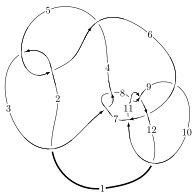
\includegraphics[width=112pt]{../../../GIT/diagram.site/Diagrams/png/2320_12n_0231.png}\\
\ \ \ A knot diagram\footnotemark}&
\allowdisplaybreaks
\textbf{Linearized knot diagam} \\
\cline{2-2}
 &
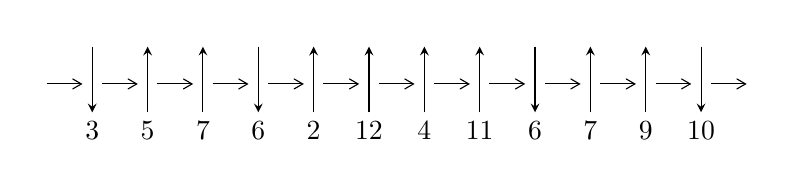
\begin{tikzpicture}[x=20pt, y=17pt]
	% nodes
	\node (C0) at (0, 0) {};
	\node (C1) at (1, 0) {};
	\node (C1U) at (1, +1) {};
	\node (C1D) at (1, -1) {3};

	\node (C2) at (2, 0) {};
	\node (C2U) at (2, +1) {};
	\node (C2D) at (2, -1) {5};

	\node (C3) at (3, 0) {};
	\node (C3U) at (3, +1) {};
	\node (C3D) at (3, -1) {7};

	\node (C4) at (4, 0) {};
	\node (C4U) at (4, +1) {};
	\node (C4D) at (4, -1) {6};

	\node (C5) at (5, 0) {};
	\node (C5U) at (5, +1) {};
	\node (C5D) at (5, -1) {2};

	\node (C6) at (6, 0) {};
	\node (C6U) at (6, +1) {};
	\node (C6D) at (6, -1) {12};

	\node (C7) at (7, 0) {};
	\node (C7U) at (7, +1) {};
	\node (C7D) at (7, -1) {4};

	\node (C8) at (8, 0) {};
	\node (C8U) at (8, +1) {};
	\node (C8D) at (8, -1) {11};

	\node (C9) at (9, 0) {};
	\node (C9U) at (9, +1) {};
	\node (C9D) at (9, -1) {6};

	\node (C10) at (10, 0) {};
	\node (C10U) at (10, +1) {};
	\node (C10D) at (10, -1) {7};

	\node (C11) at (11, 0) {};
	\node (C11U) at (11, +1) {};
	\node (C11D) at (11, -1) {9};

	\node (C12) at (12, 0) {};
	\node (C12U) at (12, +1) {};
	\node (C12D) at (12, -1) {10};
	\node (C13) at (13, 0) {};

	% arrows
	\draw[->,>={angle 60}]
	(C0) edge (C1) (C1) edge (C2) (C2) edge (C3) (C3) edge (C4) (C4) edge (C5) (C5) edge (C6) (C6) edge (C7) (C7) edge (C8) (C8) edge (C9) (C9) edge (C10) (C10) edge (C11) (C11) edge (C12) (C12) edge (C13) ;	\draw[->,>=stealth]
	(C1U) edge (C1D) (C2D) edge (C2U) (C3D) edge (C3U) (C4U) edge (C4D) (C5D) edge (C5U) (C6D) edge (C6U) (C7D) edge (C7U) (C8D) edge (C8U) (C9U) edge (C9D) (C10D) edge (C10U) (C11D) edge (C11U) (C12U) edge (C12D) ;
	\end{tikzpicture} \\
\hhline{~~} \\& 
\textbf{Solving Sequence} \\ \cline{2-2} 
 &
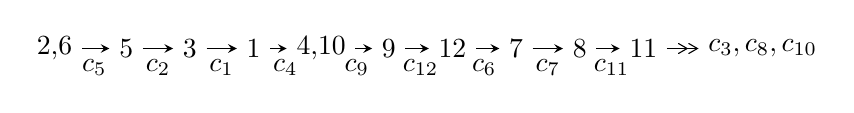
\begin{tikzpicture}[x=23pt, y=7pt]
	% node
	\node (A0) at (-1/8, 0) {2,6};
	\node (A1) at (1, 0) {5};
	\node (A2) at (2, 0) {3};
	\node (A3) at (3, 0) {1};
	\node (A4) at (65/16, 0) {4,10};
	\node (A5) at (41/8, 0) {9};
	\node (A6) at (49/8, 0) {12};
	\node (A7) at (57/8, 0) {7};
	\node (A8) at (65/8, 0) {8};
	\node (A9) at (73/8, 0) {11};
	\node (C1) at (1/2, -1) {$c_{5}$};
	\node (C2) at (3/2, -1) {$c_{2}$};
	\node (C3) at (5/2, -1) {$c_{1}$};
	\node (C4) at (7/2, -1) {$c_{4}$};
	\node (C5) at (37/8, -1) {$c_{9}$};
	\node (C6) at (45/8, -1) {$c_{12}$};
	\node (C7) at (53/8, -1) {$c_{6}$};
	\node (C8) at (61/8, -1) {$c_{7}$};
	\node (C9) at (69/8, -1) {$c_{11}$};
	\node (A10) at (11, 0) {$c_{3},c_{8},c_{10}$};

	% edge
	\draw[->,>=stealth]	
	(A0) edge (A1) (A1) edge (A2) (A2) edge (A3) (A3) edge (A4) (A4) edge (A5) (A5) edge (A6) (A6) edge (A7) (A7) edge (A8) (A8) edge (A9) ;
	\draw[->>,>={angle 60}]	
	(A9) edge (A10);
\end{tikzpicture} \\ 

\end{tabular} \\

\footnotetext{
The image of knot diagram is generated by the software ``\textbf{Draw programme}" developed by Andrew Bartholomew(\url{http://www.layer8.co.uk/maths/draw/index.htm\#Running-draw}), where we modified some parts for our purpose(\url{https://github.com/CATsTAILs/LinksPainter}).
}\phantom \\ \newline 
\centering \textbf{Ideals for irreducible components\footnotemark of $X_{\text{par}}$} 
 
\begin{align*}
I^u_{1}&=\langle 
-3.18774\times10^{22} u^{33}-2.14694\times10^{23} u^{32}+\cdots+1.21101\times10^{23} b-1.90029\times10^{23},\\
\phantom{I^u_{1}}&\phantom{= \langle  }-3.45182\times10^{23} u^{33}-2.34305\times10^{24} u^{32}+\cdots+2.42202\times10^{23} a-4.10630\times10^{23},\\
\phantom{I^u_{1}}&\phantom{= \langle  }u^{34}+7 u^{33}+\cdots-74 u^2+1\rangle \\
I^u_{2}&=\langle 
u^4+u^3+u^2+b+1,\;- u^8- u^7-2 u^6- u^5-2 u^4+a+u,\;u^9+u^8+2 u^7+u^6+3 u^5+u^4+2 u^3+u-1\rangle \\
I^u_{3}&=\langle 
85 a^4 u+42 a^4+387 a^3 u+199 a^3+170 a^2 u+84 a^2-1331 a u+661 b+641 a-639 u+563,\\
\phantom{I^u_{3}}&\phantom{= \langle  }a^5- a^4 u+6 a^4-3 a^3 u+7 a^3-4 a^2 u-2 a^2-4 a u-3 a-3 u+2,\;u^2- u+1\rangle \\
\\
\end{align*}
\raggedright * 3 irreducible components of $\dim_{\mathbb{C}}=0$, with total 53 representations.\\
\footnotetext{All coefficients of polynomials are rational numbers. But the coefficients are sometimes approximated in decimal forms when there is not enough margin.}
\newpage
\renewcommand{\arraystretch}{1}
\centering \section*{I. $I^u_{1}= \langle -3.19\times10^{22} u^{33}-2.15\times10^{23} u^{32}+\cdots+1.21\times10^{23} b-1.90\times10^{23},\;-3.45\times10^{23} u^{33}-2.34\times10^{24} u^{32}+\cdots+2.42\times10^{23} a-4.11\times10^{23},\;u^{34}+7 u^{33}+\cdots-74 u^2+1 \rangle$}
\flushleft \textbf{(i) Arc colorings}\\
\begin{tabular}{m{7pt} m{180pt} m{7pt} m{180pt} }
\flushright $a_{2}=$&$\begin{pmatrix}0\\u\end{pmatrix}$ \\
\flushright $a_{6}=$&$\begin{pmatrix}1\\0\end{pmatrix}$ \\
\flushright $a_{5}=$&$\begin{pmatrix}1\\u^2\end{pmatrix}$ \\
\flushright $a_{3}=$&$\begin{pmatrix}u\\u^3+u\end{pmatrix}$ \\
\flushright $a_{1}=$&$\begin{pmatrix}u^3\\u^5+u^3+u\end{pmatrix}$ \\
\flushright $a_{4}=$&$\begin{pmatrix}u^2+1\\u^2\end{pmatrix}$ \\
\flushright $a_{10}=$&$\begin{pmatrix}1.42518 u^{33}+9.67395 u^{32}+\cdots-42.6225 u+1.69541\\0.263230 u^{33}+1.77285 u^{32}+\cdots+0.525882 u+1.56918\end{pmatrix}$ \\
\flushright $a_{9}=$&$\begin{pmatrix}1.68841 u^{33}+11.4468 u^{32}+\cdots-42.0967 u+3.26459\\0.263230 u^{33}+1.77285 u^{32}+\cdots+0.525882 u+1.56918\end{pmatrix}$ \\
\flushright $a_{12}=$&$\begin{pmatrix}0.659832 u^{33}+4.48364 u^{32}+\cdots-8.51786 u+6.27891\\0.167487 u^{33}+1.14300 u^{32}+\cdots-7.71333 u+0.854394\end{pmatrix}$ \\
\flushright $a_{7}=$&$\begin{pmatrix}-1.00469 u^{33}-6.82609 u^{32}+\cdots+27.7668 u-2.41301\\-0.206738 u^{33}-1.42931 u^{32}+\cdots+2.41301 u-1.00469\end{pmatrix}$ \\
\flushright $a_{8}=$&$\begin{pmatrix}-1.16508 u^{33}-7.90987 u^{32}+\cdots+29.5857 u-3.25804\\-0.163277 u^{33}-1.11534 u^{32}+\cdots+2.61686 u-1.03391\end{pmatrix}$ \\
\flushright $a_{11}=$&$\begin{pmatrix}1.21680 u^{33}+8.24852 u^{32}+\cdots-28.4228 u+3.63665\\0.229994 u^{33}+1.53559 u^{32}+\cdots-1.41536 u+1.36080\end{pmatrix}$\\&\end{tabular}
\flushleft \textbf{(ii) Obstruction class $= -1$}\\~\\
\flushleft \textbf{(iii) Cusp Shapes $= -\frac{238664623265196673820757}{242201601551334258096944} u^{33}-\frac{192207794961190758657281}{30275200193916782262118} u^{32}+\cdots+\frac{3081960954854359198439141}{242201601551334258096944} u-\frac{108096673891086962943351}{30275200193916782262118}$}\\~\\
\newpage\renewcommand{\arraystretch}{1}
\flushleft \textbf{(iv) u-Polynomials at the component}\newline \\
\begin{tabular}{m{50pt}|m{274pt}}
Crossings & \hspace{64pt}u-Polynomials at each crossing \\
\hline $$\begin{aligned}c_{1},c_{4}\end{aligned}$$&$\begin{aligned}
&u^{34}+23 u^{33}+\cdots-148 u+1
\end{aligned}$\\
\hline $$\begin{aligned}c_{2},c_{5}\end{aligned}$$&$\begin{aligned}
&u^{34}+7 u^{33}+\cdots-74 u^2+1
\end{aligned}$\\
\hline $$\begin{aligned}c_{3},c_{7}\end{aligned}$$&$\begin{aligned}
&u^{34}+2 u^{33}+\cdots-3072 u+1024
\end{aligned}$\\
\hline $$\begin{aligned}c_{6}\end{aligned}$$&$\begin{aligned}
&u^{34}+4 u^{33}+\cdots-3 u-1
\end{aligned}$\\
\hline $$\begin{aligned}c_{8},c_{11}\end{aligned}$$&$\begin{aligned}
&u^{34}+12 u^{33}+\cdots-11 u-1
\end{aligned}$\\
\hline $$\begin{aligned}c_{9}\end{aligned}$$&$\begin{aligned}
&u^{34}+2 u^{33}+\cdots-10595 u+25489
\end{aligned}$\\
\hline $$\begin{aligned}c_{10}\end{aligned}$$&$\begin{aligned}
&u^{34}-4 u^{33}+\cdots-666199 u+339173
\end{aligned}$\\
\hline $$\begin{aligned}c_{12}\end{aligned}$$&$\begin{aligned}
&u^{34}-3 u^{33}+\cdots-5632 u+512
\end{aligned}$\\
\hline
\end{tabular}\\~\\
\newpage\renewcommand{\arraystretch}{1}
\flushleft \textbf{(v) Riley Polynomials at the component}\newline \\
\begin{tabular}{m{50pt}|m{274pt}}
Crossings & \hspace{64pt}Riley Polynomials at each crossing \\
\hline $$\begin{aligned}c_{1},c_{4}\end{aligned}$$&$\begin{aligned}
&y^{34}-17 y^{33}+\cdots-14096 y+1
\end{aligned}$\\
\hline $$\begin{aligned}c_{2},c_{5}\end{aligned}$$&$\begin{aligned}
&y^{34}+23 y^{33}+\cdots-148 y+1
\end{aligned}$\\
\hline $$\begin{aligned}c_{3},c_{7}\end{aligned}$$&$\begin{aligned}
&y^{34}+50 y^{33}+\cdots+1048576 y+1048576
\end{aligned}$\\
\hline $$\begin{aligned}c_{6}\end{aligned}$$&$\begin{aligned}
&y^{34}-4 y^{33}+\cdots-19 y+1
\end{aligned}$\\
\hline $$\begin{aligned}c_{8},c_{11}\end{aligned}$$&$\begin{aligned}
&y^{34}-4 y^{33}+\cdots+65 y+1
\end{aligned}$\\
\hline $$\begin{aligned}c_{9}\end{aligned}$$&$\begin{aligned}
&y^{34}-36 y^{33}+\cdots+7287355609 y+649689121
\end{aligned}$\\
\hline $$\begin{aligned}c_{10}\end{aligned}$$&$\begin{aligned}
&y^{34}+60 y^{33}+\cdots-783443850999 y+115038323929
\end{aligned}$\\
\hline $$\begin{aligned}c_{12}\end{aligned}$$&$\begin{aligned}
&y^{34}-51 y^{33}+\cdots-3407872 y+262144
\end{aligned}$\\
\hline
\end{tabular}\\~\\
\newpage\flushleft \textbf{(vi) Complex Volumes and Cusp Shapes}
$$\begin{array}{c|c|c}  
\text{Solutions to }I^u_{1}& \I (\text{vol} + \sqrt{-1}CS) & \text{Cusp shape}\\
 \hline 
\begin{aligned}
u &= \phantom{-}0.544020 + 0.828457 I \\
a &= -5.20844 + 3.26657 I \\
b &= -1.33192 + 0.57161 I\end{aligned}
 & \phantom{-}2.15188 + 2.20308 I & -18.1536 + 5.4483 I \\ \hline\begin{aligned}
u &= \phantom{-}0.544020 - 0.828457 I \\
a &= -5.20844 - 3.26657 I \\
b &= -1.33192 - 0.57161 I\end{aligned}
 & \phantom{-}2.15188 - 2.20308 I & -18.1536 - 5.4483 I \\ \hline\begin{aligned}
u &= \phantom{-}0.257238 + 0.890862 I \\
a &= -0.124907 + 0.904670 I \\
b &= \phantom{-}0.369797 + 0.819998 I\end{aligned}
 & \phantom{-}1.56878 + 0.34703 I & \phantom{-}8.40786 - 0.51532 I \\ \hline\begin{aligned}
u &= \phantom{-}0.257238 - 0.890862 I \\
a &= -0.124907 - 0.904670 I \\
b &= \phantom{-}0.369797 - 0.819998 I\end{aligned}
 & \phantom{-}1.56878 - 0.34703 I & \phantom{-}8.40786 + 0.51532 I \\ \hline\begin{aligned}
u &= -0.691884 + 0.838034 I \\
a &= \phantom{-}0.811010 + 0.201841 I \\
b &= \phantom{-}0.622736 - 0.920702 I\end{aligned}
 & \phantom{-}6.54075 + 2.05806 I & \phantom{-}13.8961 - 2.8397 I \\ \hline\begin{aligned}
u &= -0.691884 - 0.838034 I \\
a &= \phantom{-}0.811010 - 0.201841 I \\
b &= \phantom{-}0.622736 + 0.920702 I\end{aligned}
 & \phantom{-}6.54075 - 2.05806 I & \phantom{-}13.8961 + 2.8397 I \\ \hline\begin{aligned}
u &= \phantom{-}0.487947 + 1.003910 I \\
a &= -2.08476 + 1.15239 I \\
b &= \phantom{-}0.05782 - 1.46259 I\end{aligned}
 & \phantom{-}0.72250 + 2.82980 I & \phantom{-}10.05148 - 3.22591 I \\ \hline\begin{aligned}
u &= \phantom{-}0.487947 - 1.003910 I \\
a &= -2.08476 - 1.15239 I \\
b &= \phantom{-}0.05782 + 1.46259 I\end{aligned}
 & \phantom{-}0.72250 - 2.82980 I & \phantom{-}10.05148 + 3.22591 I \\ \hline\begin{aligned}
u &= \phantom{-}0.657459 + 0.922088 I \\
a &= -0.764190 + 0.647851 I \\
b &= -0.691749 - 0.367275 I\end{aligned}
 & \phantom{-}0.62542 + 2.57137 I & \phantom{-}3.17282 - 2.86214 I \\ \hline\begin{aligned}
u &= \phantom{-}0.657459 - 0.922088 I \\
a &= -0.764190 - 0.647851 I \\
b &= -0.691749 + 0.367275 I\end{aligned}
 & \phantom{-}0.62542 - 2.57137 I & \phantom{-}3.17282 + 2.86214 I\\
 \hline 
 \end{array}$$\newpage$$\begin{array}{c|c|c}  
\text{Solutions to }I^u_{1}& \I (\text{vol} + \sqrt{-1}CS) & \text{Cusp shape}\\
 \hline 
\begin{aligned}
u &= \phantom{-}0.175415 + 0.847114 I \\
a &= \phantom{-}0.046460 - 1.237630 I \\
b &= -0.115474 + 0.349761 I\end{aligned}
 & -1.59132 + 1.76956 I & -2.73476 - 4.21364 I \\ \hline\begin{aligned}
u &= \phantom{-}0.175415 - 0.847114 I \\
a &= \phantom{-}0.046460 + 1.237630 I \\
b &= -0.115474 - 0.349761 I\end{aligned}
 & -1.59132 - 1.76956 I & -2.73476 + 4.21364 I \\ \hline\begin{aligned}
u &= -1.132310 + 0.183127 I \\
a &= \phantom{-}0.002681 - 0.231147 I \\
b &= \phantom{-}1.39864 - 0.29584 I\end{aligned}
 & -7.72558 + 0.90268 I & \phantom{-}5.49060 + 0.21802 I \\ \hline\begin{aligned}
u &= -1.132310 - 0.183127 I \\
a &= \phantom{-}0.002681 + 0.231147 I \\
b &= \phantom{-}1.39864 + 0.29584 I\end{aligned}
 & -7.72558 - 0.90268 I & \phantom{-}5.49060 - 0.21802 I \\ \hline\begin{aligned}
u &= -0.623744 + 0.978086 I \\
a &= -0.574996 + 0.242105 I \\
b &= \phantom{-}0.236214 + 0.979802 I\end{aligned}
 & \phantom{-}6.07730 - 7.11588 I & \phantom{-}12.1179 + 9.6630 I \\ \hline\begin{aligned}
u &= -0.623744 - 0.978086 I \\
a &= -0.574996 - 0.242105 I \\
b &= \phantom{-}0.236214 - 0.979802 I\end{aligned}
 & \phantom{-}6.07730 + 7.11588 I & \phantom{-}12.1179 - 9.6630 I \\ \hline\begin{aligned}
u &= -1.215360 + 0.226914 I \\
a &= -0.352940 + 0.538182 I \\
b &= -2.06341 + 1.43354 I\end{aligned}
 & -7.46169 + 8.00267 I & \phantom{-}5.84717 - 3.91358 I \\ \hline\begin{aligned}
u &= -1.215360 - 0.226914 I \\
a &= -0.352940 - 0.538182 I \\
b &= -2.06341 - 1.43354 I\end{aligned}
 & -7.46169 - 8.00267 I & \phantom{-}5.84717 + 3.91358 I \\ \hline\begin{aligned}
u &= -0.021777 + 1.291760 I \\
a &= \phantom{-}1.45710 + 0.36632 I \\
b &= -0.94260 - 1.15777 I\end{aligned}
 & -2.99715 - 2.34695 I & \phantom{-}2.86038 + 3.07511 I \\ \hline\begin{aligned}
u &= -0.021777 - 1.291760 I \\
a &= \phantom{-}1.45710 - 0.36632 I \\
b &= -0.94260 + 1.15777 I\end{aligned}
 & -2.99715 + 2.34695 I & \phantom{-}2.86038 - 3.07511 I\\
 \hline 
 \end{array}$$\newpage$$\begin{array}{c|c|c}  
\text{Solutions to }I^u_{1}& \I (\text{vol} + \sqrt{-1}CS) & \text{Cusp shape}\\
 \hline 
\begin{aligned}
u &= \phantom{-}0.649185\phantom{ +0.000000I} \\
a &= -0.175240\phantom{ +0.000000I} \\
b &= \phantom{-}0.825508\phantom{ +0.000000I}\end{aligned}
 & \phantom{-}1.38631\phantom{ +0.000000I} & \phantom{-}7.11490\phantom{ +0.000000I} \\ \hline\begin{aligned}
u &= \phantom{-}0.15024 + 1.45013 I \\
a &= -1.66300 - 0.69317 I \\
b &= \phantom{-}2.33781 + 0.73216 I\end{aligned}
 & -3.63061 + 2.77360 I & \phantom{-0.000000 } 0 \\ \hline\begin{aligned}
u &= \phantom{-}0.15024 - 1.45013 I \\
a &= -1.66300 + 0.69317 I \\
b &= \phantom{-}2.33781 - 0.73216 I\end{aligned}
 & -3.63061 - 2.77360 I & \phantom{-0.000000 } 0 \\ \hline\begin{aligned}
u &= -0.65730 + 1.31359 I \\
a &= -1.22670 + 0.80696 I \\
b &= \phantom{-}1.26804 + 0.74707 I\end{aligned}
 & -11.18750 - 7.23815 I & \phantom{-0.000000 } 0 \\ \hline\begin{aligned}
u &= -0.65730 - 1.31359 I \\
a &= -1.22670 - 0.80696 I \\
b &= \phantom{-}1.26804 - 0.74707 I\end{aligned}
 & -11.18750 + 7.23815 I & \phantom{-0.000000 } 0 \\ \hline\begin{aligned}
u &= -0.69399 + 1.33382 I \\
a &= \phantom{-}1.80696 - 0.87095 I \\
b &= -1.73482 - 1.78350 I\end{aligned}
 & -10.8926 - 14.7212 I & \phantom{-0.000000 } 0 \\ \hline\begin{aligned}
u &= -0.69399 - 1.33382 I \\
a &= \phantom{-}1.80696 + 0.87095 I \\
b &= -1.73482 + 1.78350 I\end{aligned}
 & -10.8926 + 14.7212 I & \phantom{-0.000000 } 0 \\ \hline\begin{aligned}
u &= -0.46062 + 1.48862 I \\
a &= -1.34753 + 0.57888 I \\
b &= \phantom{-}1.88206 + 0.20245 I\end{aligned}
 & -13.09350 - 4.80207 I & \phantom{-0.000000 } 0 \\ \hline\begin{aligned}
u &= -0.46062 - 1.48862 I \\
a &= -1.34753 - 0.57888 I \\
b &= \phantom{-}1.88206 - 0.20245 I\end{aligned}
 & -13.09350 + 4.80207 I & \phantom{-0.000000 } 0 \\ \hline\begin{aligned}
u &= -0.43913 + 1.57970 I \\
a &= \phantom{-}1.14509 - 1.20205 I \\
b &= -2.89525 + 1.03267 I\end{aligned}
 & -13.37580 + 1.94532 I & \phantom{-0.000000 } 0\\
 \hline 
 \end{array}$$\newpage$$\begin{array}{c|c|c}  
\text{Solutions to }I^u_{1}& \I (\text{vol} + \sqrt{-1}CS) & \text{Cusp shape}\\
 \hline 
\begin{aligned}
u &= -0.43913 - 1.57970 I \\
a &= \phantom{-}1.14509 + 1.20205 I \\
b &= -2.89525 - 1.03267 I\end{aligned}
 & -13.37580 - 1.94532 I & \phantom{-0.000000 } 0 \\ \hline\begin{aligned}
u &= -0.207141 + 0.051709 I \\
a &= -1.65437 + 3.73289 I \\
b &= -0.331665 + 0.940404 I\end{aligned}
 & \phantom{-}0.61291 + 1.48611 I & \phantom{-}4.79533 - 4.74523 I \\ \hline\begin{aligned}
u &= -0.207141 - 0.051709 I \\
a &= -1.65437 - 3.73289 I \\
b &= -0.331665 - 0.940404 I\end{aligned}
 & \phantom{-}0.61291 - 1.48611 I & \phantom{-}4.79533 + 4.74523 I \\ \hline\begin{aligned}
u &= \phantom{-}0.0926838\phantom{ +0.000000I} \\
a &= -6.35971\phantom{ +0.000000I} \\
b &= \phantom{-}1.04203\phantom{ +0.000000I}\end{aligned}
 & \phantom{-}2.29528\phantom{ +0.000000I} & \phantom{-}1.25710\phantom{ +0.000000I}\\
 \hline 
 \end{array}$$\newpage\newpage\renewcommand{\arraystretch}{1}
\centering \section*{II. $I^u_{2}= \langle u^4+u^3+u^2+b+1,\;- u^8- u^7-2 u^6- u^5-2 u^4+a+u,\;u^9+u^8+2 u^7+u^6+3 u^5+u^4+2 u^3+u-1 \rangle$}
\flushleft \textbf{(i) Arc colorings}\\
\begin{tabular}{m{7pt} m{180pt} m{7pt} m{180pt} }
\flushright $a_{2}=$&$\begin{pmatrix}0\\u\end{pmatrix}$ \\
\flushright $a_{6}=$&$\begin{pmatrix}1\\0\end{pmatrix}$ \\
\flushright $a_{5}=$&$\begin{pmatrix}1\\u^2\end{pmatrix}$ \\
\flushright $a_{3}=$&$\begin{pmatrix}u\\u^3+u\end{pmatrix}$ \\
\flushright $a_{1}=$&$\begin{pmatrix}u^3\\u^5+u^3+u\end{pmatrix}$ \\
\flushright $a_{4}=$&$\begin{pmatrix}u^2+1\\u^2\end{pmatrix}$ \\
\flushright $a_{10}=$&$\begin{pmatrix}u^8+u^7+2 u^6+u^5+2 u^4- u\\- u^4- u^3- u^2-1\end{pmatrix}$ \\
\flushright $a_{9}=$&$\begin{pmatrix}u^8+u^7+2 u^6+u^5+u^4- u^3- u^2- u-1\\- u^4- u^3- u^2-1\end{pmatrix}$ \\
\flushright $a_{12}=$&$\begin{pmatrix}u^3\\u^5+u^3+u\end{pmatrix}$ \\
\flushright $a_{7}=$&$\begin{pmatrix}- u^8- u^6- u^4+1\\- u^8- u^7- u^6-2 u^5- u^4-2 u^3-2 u+1\end{pmatrix}$ \\
\flushright $a_{8}=$&$\begin{pmatrix}- u^3\\- u^5- u^3- u\end{pmatrix}$ \\
\flushright $a_{11}=$&$\begin{pmatrix}u^8+u^7+2 u^6+u^5+u^4- u^2- u-1\\u^5- u^4- u^2+u-1\end{pmatrix}$\\&\end{tabular}
\flushleft \textbf{(ii) Obstruction class $= 1$}\\~\\
\flushleft \textbf{(iii) Cusp Shapes $= 3 u^8+9 u^7+12 u^6+13 u^5+15 u^4+15 u^3+8 u^2+5 u+9$}\\~\\
\newpage\renewcommand{\arraystretch}{1}
\flushleft \textbf{(iv) u-Polynomials at the component}\newline \\
\begin{tabular}{m{50pt}|m{274pt}}
Crossings & \hspace{64pt}u-Polynomials at each crossing \\
\hline $$\begin{aligned}c_{1},c_{4}\end{aligned}$$&$\begin{aligned}
&u^9-3 u^8+8 u^7-13 u^6+17 u^5-17 u^4+12 u^3-6 u^2+u+1
\end{aligned}$\\
\hline $$\begin{aligned}c_{2}\end{aligned}$$&$\begin{aligned}
&u^9- u^8+2 u^7- u^6+3 u^5- u^4+2 u^3+u+1
\end{aligned}$\\
\hline $$\begin{aligned}c_{3}\end{aligned}$$&$\begin{aligned}
&u^9- u^8-2 u^7+3 u^6+u^5-3 u^4+2 u^3- u+1
\end{aligned}$\\
\hline $$\begin{aligned}c_{5}\end{aligned}$$&$\begin{aligned}
&u^9+u^8+2 u^7+u^6+3 u^5+u^4+2 u^3+u-1
\end{aligned}$\\
\hline $$\begin{aligned}c_{6}\end{aligned}$$&$\begin{aligned}
&u^9-5 u^8+12 u^7-15 u^6+9 u^5+u^4-4 u^3+2 u^2+u-1
\end{aligned}$\\
\hline $$\begin{aligned}c_{7}\end{aligned}$$&$\begin{aligned}
&u^9+u^8-2 u^7-3 u^6+u^5+3 u^4+2 u^3- u-1
\end{aligned}$\\
\hline $$\begin{aligned}c_{8}\end{aligned}$$&$\begin{aligned}
&(u+1)^9
\end{aligned}$\\
\hline $$\begin{aligned}c_{9},c_{10}\end{aligned}$$&$\begin{aligned}
&u^9- u^8-2 u^7+4 u^6- u^5-9 u^4+15 u^3-12 u^2+5 u-1
\end{aligned}$\\
\hline $$\begin{aligned}c_{11}\end{aligned}$$&$\begin{aligned}
&(u-1)^9
\end{aligned}$\\
\hline $$\begin{aligned}c_{12}\end{aligned}$$&$\begin{aligned}
&u^9
\end{aligned}$\\
\hline
\end{tabular}\\~\\
\newpage\renewcommand{\arraystretch}{1}
\flushleft \textbf{(v) Riley Polynomials at the component}\newline \\
\begin{tabular}{m{50pt}|m{274pt}}
Crossings & \hspace{64pt}Riley Polynomials at each crossing \\
\hline $$\begin{aligned}c_{1},c_{4}\end{aligned}$$&$\begin{aligned}
&y^9+7 y^8+20 y^7+25 y^6+5 y^5-15 y^4+22 y^2+13 y-1
\end{aligned}$\\
\hline $$\begin{aligned}c_{2},c_{5}\end{aligned}$$&$\begin{aligned}
&y^9+3 y^8+8 y^7+13 y^6+17 y^5+17 y^4+12 y^3+6 y^2+y-1
\end{aligned}$\\
\hline $$\begin{aligned}c_{3},c_{7}\end{aligned}$$&$\begin{aligned}
&y^9-5 y^8+12 y^7-15 y^6+9 y^5+y^4-4 y^3+2 y^2+y-1
\end{aligned}$\\
\hline $$\begin{aligned}c_{6}\end{aligned}$$&$\begin{aligned}
&y^9- y^8+12 y^7-7 y^6+37 y^5+y^4-10 y^2+5 y-1
\end{aligned}$\\
\hline $$\begin{aligned}c_{8},c_{11}\end{aligned}$$&$\begin{aligned}
&(y-1)^9
\end{aligned}$\\
\hline $$\begin{aligned}c_{9},c_{10}\end{aligned}$$&$\begin{aligned}
&y^9-5 y^8+10 y^7- y^5-37 y^4+7 y^3-12 y^2+y-1
\end{aligned}$\\
\hline $$\begin{aligned}c_{12}\end{aligned}$$&$\begin{aligned}
&y^9
\end{aligned}$\\
\hline
\end{tabular}\\~\\
\newpage\flushleft \textbf{(vi) Complex Volumes and Cusp Shapes}
$$\begin{array}{c|c|c}  
\text{Solutions to }I^u_{2}& \I (\text{vol} + \sqrt{-1}CS) & \text{Cusp shape}\\
 \hline 
\begin{aligned}
u &= \phantom{-}0.140343 + 0.966856 I \\
a &= \phantom{-}0.463951 - 1.179170 I \\
b &= -0.457852 + 1.072010 I\end{aligned}
 & -0.13850 + 2.09337 I & \phantom{-}3.38047 - 2.85927 I \\ \hline\begin{aligned}
u &= \phantom{-}0.140343 - 0.966856 I \\
a &= \phantom{-}0.463951 + 1.179170 I \\
b &= -0.457852 - 1.072010 I\end{aligned}
 & -0.13850 - 2.09337 I & \phantom{-}3.38047 + 2.85927 I \\ \hline\begin{aligned}
u &= \phantom{-}0.628449 + 0.875112 I \\
a &= \phantom{-}1.92263 - 3.37970 I \\
b &= \phantom{-}1.63880 - 0.65075 I\end{aligned}
 & \phantom{-}2.26187 + 2.45442 I & \phantom{-}6.9022 - 12.4598 I \\ \hline\begin{aligned}
u &= \phantom{-}0.628449 - 0.875112 I \\
a &= \phantom{-}1.92263 + 3.37970 I \\
b &= \phantom{-}1.63880 + 0.65075 I\end{aligned}
 & \phantom{-}2.26187 - 2.45442 I & \phantom{-}6.9022 + 12.4598 I \\ \hline\begin{aligned}
u &= -0.796005 + 0.733148 I \\
a &= -0.502055 + 0.200019 I \\
b &= -0.522253 + 0.392004 I\end{aligned}
 & \phantom{-}6.01628 + 1.33617 I & \phantom{-}6.48878 + 2.15019 I \\ \hline\begin{aligned}
u &= -0.796005 - 0.733148 I \\
a &= -0.502055 - 0.200019 I \\
b &= -0.522253 - 0.392004 I\end{aligned}
 & \phantom{-}6.01628 - 1.33617 I & \phantom{-}6.48878 - 2.15019 I \\ \hline\begin{aligned}
u &= -0.728966 + 0.986295 I \\
a &= \phantom{-}0.259988 - 0.648365 I \\
b &= -0.425734 - 0.444312 I\end{aligned}
 & \phantom{-}5.24306 - 7.08493 I & \phantom{-}2.48514 + 6.49599 I \\ \hline\begin{aligned}
u &= -0.728966 - 0.986295 I \\
a &= \phantom{-}0.259988 + 0.648365 I \\
b &= -0.425734 + 0.444312 I\end{aligned}
 & \phantom{-}5.24306 + 7.08493 I & \phantom{-}2.48514 - 6.49599 I \\ \hline\begin{aligned}
u &= \phantom{-}0.512358\phantom{ +0.000000I} \\
a &= -0.289029\phantom{ +0.000000I} \\
b &= -1.46592\phantom{ +0.000000I}\end{aligned}
 & \phantom{-}2.84338\phantom{ +0.000000I} & \phantom{-}17.4870\phantom{ +0.000000I}\\
 \hline 
 \end{array}$$\newpage\newpage\renewcommand{\arraystretch}{1}
\centering \section*{III. $I^u_{3}= \langle 85 a^4 u+387 a^3 u+\cdots+641 a+563,\;- a^4 u-3 a^3 u+\cdots-3 a+2,\;u^2- u+1 \rangle$}
\flushleft \textbf{(i) Arc colorings}\\
\begin{tabular}{m{7pt} m{180pt} m{7pt} m{180pt} }
\flushright $a_{2}=$&$\begin{pmatrix}0\\u\end{pmatrix}$ \\
\flushright $a_{6}=$&$\begin{pmatrix}1\\0\end{pmatrix}$ \\
\flushright $a_{5}=$&$\begin{pmatrix}1\\u-1\end{pmatrix}$ \\
\flushright $a_{3}=$&$\begin{pmatrix}u\\u-1\end{pmatrix}$ \\
\flushright $a_{1}=$&$\begin{pmatrix}-1\\0\end{pmatrix}$ \\
\flushright $a_{4}=$&$\begin{pmatrix}u\\u-1\end{pmatrix}$ \\
\flushright $a_{10}=$&$\begin{pmatrix}a\\-0.128593 a^{4} u-0.585477 a^{3} u+\cdots-0.969743 a-0.851740\end{pmatrix}$ \\
\flushright $a_{9}=$&$\begin{pmatrix}-0.128593 a^{4} u-0.585477 a^{3} u+\cdots+0.0302572 a-0.851740\\-0.128593 a^{4} u-0.585477 a^{3} u+\cdots-0.969743 a-0.851740\end{pmatrix}$ \\
\flushright $a_{12}=$&$\begin{pmatrix}-0.00605144 a^{4} u+0.0665658 a^{3} u+\cdots-0.527988 a-0.487141\\0.337368 a^{4} u+1.28896 a^{3} u+\cdots+0.685325 a-0.341906\end{pmatrix}$ \\
\flushright $a_{7}=$&$\begin{pmatrix}0.0862330 a^{4} u+0.0514372 a^{3} u+\cdots-2.72617 a+1.44175\\0.611195 a^{4} u+2.27685 a^{3} u+\cdots+1.32678 a+1.20121\end{pmatrix}$ \\
\flushright $a_{8}=$&$\begin{pmatrix}0.0862330 a^{4} u+0.0514372 a^{3} u+\cdots-2.72617 a+1.44175\\0.611195 a^{4} u+2.27685 a^{3} u+\cdots+1.32678 a+1.20121\end{pmatrix}$ \\
\flushright $a_{11}=$&$\begin{pmatrix}0.0226929 a^{4} u-0.249622 a^{3} u+\cdots-2.77005 a+1.32678\\0.611195 a^{4} u+2.27685 a^{3} u+\cdots+1.32678 a+1.20121\end{pmatrix}$\\&\end{tabular}
\flushleft \textbf{(ii) Obstruction class $= 1$}\\~\\
\flushleft \textbf{(iii) Cusp Shapes $= \frac{1623}{661} a^4 u+\frac{522}{661} a^4+\frac{5282}{661} a^3 u+\frac{4173}{661} a^3-\frac{2703}{661} a^2 u+\frac{3688}{661} a^2-\frac{9177}{661} a u+\frac{2301}{661} a-\frac{2465}{661} u+\frac{6714}{661}$}\\~\\
\newpage\renewcommand{\arraystretch}{1}
\flushleft \textbf{(iv) u-Polynomials at the component}\newline \\
\begin{tabular}{m{50pt}|m{274pt}}
Crossings & \hspace{64pt}u-Polynomials at each crossing \\
\hline $$\begin{aligned}c_{1},c_{4},c_{5}\end{aligned}$$&$\begin{aligned}
&(u^2- u+1)^5
\end{aligned}$\\
\hline $$\begin{aligned}c_{2}\end{aligned}$$&$\begin{aligned}
&(u^2+u+1)^5
\end{aligned}$\\
\hline $$\begin{aligned}c_{3},c_{7}\end{aligned}$$&$\begin{aligned}
&u^{10}
\end{aligned}$\\
\hline $$\begin{aligned}c_{6}\end{aligned}$$&$\begin{aligned}
&(u^5+3 u^4+4 u^3+u^2- u-1)^2
\end{aligned}$\\
\hline $$\begin{aligned}c_{8}\end{aligned}$$&$\begin{aligned}
&(u^5- u^4-2 u^3+u^2+u+1)^2
\end{aligned}$\\
\hline $$\begin{aligned}c_{9},c_{12}\end{aligned}$$&$\begin{aligned}
&(u^5- u^4+2 u^3- u^2+u-1)^2
\end{aligned}$\\
\hline $$\begin{aligned}c_{10},c_{11}\end{aligned}$$&$\begin{aligned}
&(u^5+u^4-2 u^3- u^2+u-1)^2
\end{aligned}$\\
\hline
\end{tabular}\\~\\
\newpage\renewcommand{\arraystretch}{1}
\flushleft \textbf{(v) Riley Polynomials at the component}\newline \\
\begin{tabular}{m{50pt}|m{274pt}}
Crossings & \hspace{64pt}Riley Polynomials at each crossing \\
\hline $$\begin{aligned}c_{1},c_{2},c_{4}\\c_{5}\end{aligned}$$&$\begin{aligned}
&(y^2+y+1)^5
\end{aligned}$\\
\hline $$\begin{aligned}c_{3},c_{7}\end{aligned}$$&$\begin{aligned}
&y^{10}
\end{aligned}$\\
\hline $$\begin{aligned}c_{6}\end{aligned}$$&$\begin{aligned}
&(y^5- y^4+8 y^3-3 y^2+3 y-1)^2
\end{aligned}$\\
\hline $$\begin{aligned}c_{8},c_{10},c_{11}\end{aligned}$$&$\begin{aligned}
&(y^5-5 y^4+8 y^3-3 y^2- y-1)^2
\end{aligned}$\\
\hline $$\begin{aligned}c_{9},c_{12}\end{aligned}$$&$\begin{aligned}
&(y^5+3 y^4+4 y^3+y^2- y-1)^2
\end{aligned}$\\
\hline
\end{tabular}\\~\\
\newpage\flushleft \textbf{(vi) Complex Volumes and Cusp Shapes}
$$\begin{array}{c|c|c}  
\text{Solutions to }I^u_{3}& \I (\text{vol} + \sqrt{-1}CS) & \text{Cusp shape}\\
 \hline 
\begin{aligned}
u &= \phantom{-}0.500000 + 0.866025 I \\
a &= \phantom{-}0.953786 + 0.485650 I \\
b &= -0.455697 + 1.200150 I\end{aligned}
 & \phantom{-}5.87256 + 6.43072 I & \phantom{-}6.63163 - 0.01393 I \\ \hline\begin{aligned}
u &= \phantom{-}0.500000 + 0.866025 I \\
a &= -1.124940 + 0.303641 I \\
b &= -0.455697 - 1.200150 I\end{aligned}
 & \phantom{-}5.87256 - 2.37095 I & \phantom{-}3.55752 + 5.27247 I \\ \hline\begin{aligned}
u &= \phantom{-}0.500000 + 0.866025 I \\
a &= -1.42401 - 0.21550 I \\
b &= \phantom{-}0.339110 - 0.822375 I\end{aligned}
 & \phantom{-}0.32910 + 3.56046 I & \phantom{-}3.07628 - 9.77765 I \\ \hline\begin{aligned}
u &= \phantom{-}0.500000 + 0.866025 I \\
a &= \phantom{-}0.000387 - 0.371855 I \\
b &= \phantom{-}0.339110 + 0.822375 I\end{aligned}
 & \phantom{-}0.329100 + 0.499304 I & \phantom{-}3.01153 - 0.88894 I \\ \hline\begin{aligned}
u &= \phantom{-}0.500000 + 0.866025 I \\
a &= -3.90523 + 0.66409 I \\
b &= -0.766826\phantom{ +0.000000I}\end{aligned}
 & \phantom{-}2.40108 + 2.02988 I & \phantom{-}9.72304 + 3.67600 I \\ \hline\begin{aligned}
u &= \phantom{-}0.500000 - 0.866025 I \\
a &= \phantom{-}0.953786 - 0.485650 I \\
b &= -0.455697 - 1.200150 I\end{aligned}
 & \phantom{-}5.87256 - 6.43072 I & \phantom{-}6.63163 + 0.01393 I \\ \hline\begin{aligned}
u &= \phantom{-}0.500000 - 0.866025 I \\
a &= -1.124940 - 0.303641 I \\
b &= -0.455697 + 1.200150 I\end{aligned}
 & \phantom{-}5.87256 + 2.37095 I & \phantom{-}3.55752 - 5.27247 I \\ \hline\begin{aligned}
u &= \phantom{-}0.500000 - 0.866025 I \\
a &= -1.42401 + 0.21550 I \\
b &= \phantom{-}0.339110 + 0.822375 I\end{aligned}
 & \phantom{-}0.32910 - 3.56046 I & \phantom{-}3.07628 + 9.77765 I \\ \hline\begin{aligned}
u &= \phantom{-}0.500000 - 0.866025 I \\
a &= \phantom{-}0.000387 + 0.371855 I \\
b &= \phantom{-}0.339110 - 0.822375 I\end{aligned}
 & \phantom{-}0.329100 - 0.499304 I & \phantom{-}3.01153 + 0.88894 I \\ \hline\begin{aligned}
u &= \phantom{-}0.500000 - 0.866025 I \\
a &= -3.90523 - 0.66409 I \\
b &= -0.766826\phantom{ +0.000000I}\end{aligned}
 & \phantom{-}2.40108 - 2.02988 I & \phantom{-}9.72304 - 3.67600 I\\
 \hline 
 \end{array}$$\newpage
\newpage\renewcommand{\arraystretch}{1}
\centering \section*{ IV. u-Polynomials}
\begin{tabular}{m{50pt}|m{274pt}}
Crossings & \hspace{64pt}u-Polynomials at each crossing \\
\hline $$\begin{aligned}c_{1},c_{4}\end{aligned}$$&$\begin{aligned}
&(u^2- u+1)^5\\
&\cdot(u^9-3 u^8+8 u^7-13 u^6+17 u^5-17 u^4+12 u^3-6 u^2+u+1)\\
&\cdot(u^{34}+23 u^{33}+\cdots-148 u+1)
\end{aligned}$\\
\hline $$\begin{aligned}c_{2}\end{aligned}$$&$\begin{aligned}
&(u^2+u+1)^5(u^9- u^8+2 u^7- u^6+3 u^5- u^4+2 u^3+u+1)\\
&\cdot(u^{34}+7 u^{33}+\cdots-74 u^2+1)
\end{aligned}$\\
\hline $$\begin{aligned}c_{3}\end{aligned}$$&$\begin{aligned}
&u^{10}(u^9- u^8-2 u^7+3 u^6+u^5-3 u^4+2 u^3- u+1)\\
&\cdot(u^{34}+2 u^{33}+\cdots-3072 u+1024)
\end{aligned}$\\
\hline $$\begin{aligned}c_{5}\end{aligned}$$&$\begin{aligned}
&(u^2- u+1)^5(u^9+u^8+2 u^7+u^6+3 u^5+u^4+2 u^3+u-1)\\
&\cdot(u^{34}+7 u^{33}+\cdots-74 u^2+1)
\end{aligned}$\\
\hline $$\begin{aligned}c_{6}\end{aligned}$$&$\begin{aligned}
&(u^5+3 u^4+4 u^3+u^2- u-1)^2\\
&\cdot(u^9-5 u^8+12 u^7-15 u^6+9 u^5+u^4-4 u^3+2 u^2+u-1)\\
&\cdot(u^{34}+4 u^{33}+\cdots-3 u-1)
\end{aligned}$\\
\hline $$\begin{aligned}c_{7}\end{aligned}$$&$\begin{aligned}
&u^{10}(u^9+u^8-2 u^7-3 u^6+u^5+3 u^4+2 u^3- u-1)\\
&\cdot(u^{34}+2 u^{33}+\cdots-3072 u+1024)
\end{aligned}$\\
\hline $$\begin{aligned}c_{8}\end{aligned}$$&$\begin{aligned}
&((u+1)^9)(u^5- u^4+\cdots+u+1)^{2}(u^{34}+12 u^{33}+\cdots-11 u-1)
\end{aligned}$\\
\hline $$\begin{aligned}c_{9}\end{aligned}$$&$\begin{aligned}
&(u^5- u^4+2 u^3- u^2+u-1)^2\\
&\cdot(u^9- u^8-2 u^7+4 u^6- u^5-9 u^4+15 u^3-12 u^2+5 u-1)\\
&\cdot(u^{34}+2 u^{33}+\cdots-10595 u+25489)
\end{aligned}$\\
\hline $$\begin{aligned}c_{10}\end{aligned}$$&$\begin{aligned}
&(u^5+u^4-2 u^3- u^2+u-1)^2\\
&\cdot(u^9- u^8-2 u^7+4 u^6- u^5-9 u^4+15 u^3-12 u^2+5 u-1)\\
&\cdot(u^{34}-4 u^{33}+\cdots-666199 u+339173)
\end{aligned}$\\
\hline $$\begin{aligned}c_{11}\end{aligned}$$&$\begin{aligned}
&((u-1)^9)(u^5+u^4+\cdots+u-1)^{2}(u^{34}+12 u^{33}+\cdots-11 u-1)
\end{aligned}$\\
\hline $$\begin{aligned}c_{12}\end{aligned}$$&$\begin{aligned}
&u^9(u^5- u^4+\cdots+u-1)^{2}(u^{34}-3 u^{33}+\cdots-5632 u+512)
\end{aligned}$\\
\hline
\end{tabular}\newpage\renewcommand{\arraystretch}{1}
\centering \section*{ V. Riley Polynomials}
\begin{tabular}{m{50pt}|m{274pt}}
Crossings & \hspace{64pt}Riley Polynomials at each crossing \\
\hline $$\begin{aligned}c_{1},c_{4}\end{aligned}$$&$\begin{aligned}
&((y^2+y+1)^5)(y^9+7 y^8+\cdots+13 y-1)\\
&\cdot(y^{34}-17 y^{33}+\cdots-14096 y+1)
\end{aligned}$\\
\hline $$\begin{aligned}c_{2},c_{5}\end{aligned}$$&$\begin{aligned}
&(y^2+y+1)^5\\
&\cdot(y^9+3 y^8+8 y^7+13 y^6+17 y^5+17 y^4+12 y^3+6 y^2+y-1)\\
&\cdot(y^{34}+23 y^{33}+\cdots-148 y+1)
\end{aligned}$\\
\hline $$\begin{aligned}c_{3},c_{7}\end{aligned}$$&$\begin{aligned}
&y^{10}(y^9-5 y^8+12 y^7-15 y^6+9 y^5+y^4-4 y^3+2 y^2+y-1)\\
&\cdot(y^{34}+50 y^{33}+\cdots+1048576 y+1048576)
\end{aligned}$\\
\hline $$\begin{aligned}c_{6}\end{aligned}$$&$\begin{aligned}
&(y^5- y^4+8 y^3-3 y^2+3 y-1)^2\\
&\cdot(y^9- y^8+12 y^7-7 y^6+37 y^5+y^4-10 y^2+5 y-1)\\
&\cdot(y^{34}-4 y^{33}+\cdots-19 y+1)
\end{aligned}$\\
\hline $$\begin{aligned}c_{8},c_{11}\end{aligned}$$&$\begin{aligned}
&((y-1)^9)(y^5-5 y^4+\cdots- y-1)^{2}(y^{34}-4 y^{33}+\cdots+65 y+1)
\end{aligned}$\\
\hline $$\begin{aligned}c_{9}\end{aligned}$$&$\begin{aligned}
&(y^5+3 y^4+4 y^3+y^2- y-1)^2\\
&\cdot(y^9-5 y^8+10 y^7- y^5-37 y^4+7 y^3-12 y^2+y-1)\\
&\cdot(y^{34}-36 y^{33}+\cdots+7287355609 y+649689121)
\end{aligned}$\\
\hline $$\begin{aligned}c_{10}\end{aligned}$$&$\begin{aligned}
&(y^5-5 y^4+8 y^3-3 y^2- y-1)^2\\
&\cdot(y^9-5 y^8+10 y^7- y^5-37 y^4+7 y^3-12 y^2+y-1)\\
&\cdot(y^{34}+60 y^{33}+\cdots-783443850999 y+115038323929)
\end{aligned}$\\
\hline $$\begin{aligned}c_{12}\end{aligned}$$&$\begin{aligned}
&y^9(y^5+3 y^4+4 y^3+y^2- y-1)^2\\
&\cdot(y^{34}-51 y^{33}+\cdots-3407872 y+262144)
\end{aligned}$\\
\hline
\end{tabular}
\vskip 2pc
\end{document}